\section{VC Dimension [45 points]}
\label{sec:vc-dimension}
\begin{enumerate}
\item ~[5 points] Assume that the three points below can be labeled in any way.  Show with pictures how they can be shattered by a linear classifier.  Use filled dots to represent positive classes and unfilled dots to represent negative classes.

  \begin{tikzpicture}
    \begin{axis}[my style, xtick={-1,0,...,3}, ytick={-1,0,...,3},
      xmin=-1, xmax=3, ymin=-1, ymax=3]
      \addplot[mark=*,only marks] coordinates {(2,2)(1,1)(1,2)};
    \end{axis}
  \end{tikzpicture}
  
  \textbf{Response:} Refer to figure below for a visualization of a linear classifier shattering this dataset. \newline
  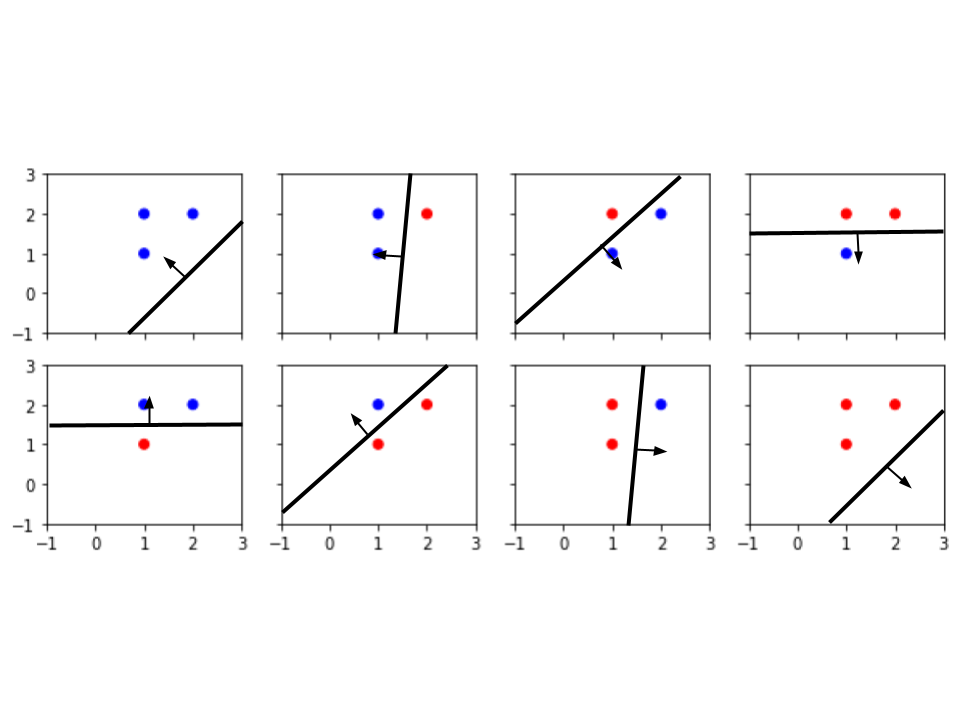
\includegraphics[scale=0.4]{./img/part3_1.png}
  
\item {\bf VC-dimension of axis aligned rectangles in $\mathbb{R}^d$}:
  Let $H^d_{rec}$ be the class of axis-aligned rectangles in
  $\mathbb{R}^d$. When $d=2$, this class simply consists of rectangles
  on the plane, and labels all points strictly outside the rectangle
  as negative and all points on or inside the rectangle as positive.
  In higher dimensions, this generalizes to $d$-dimensional boxes,
  with points outside the box labeled negative.

  \begin{enumerate}
  \item ~[10 points] Show that the VC dimension of $H^2_{rec}$ is 4.
  
  \textbf{Response:} To prove that the VC dimension of $H^2_{rec}$ is 4, $H^2_{rec}$ must shatter at least one subset of size 4 (ie, $VC(H^2_{rec}) \geq 4$) but there must not exist a single subset of size 5 that $VC(H^2_{rec})$ can shatter so $VC(H^2_{rec}) < 5$.
  \begin{enumerate}
  	\item ~Direct proof for $VC(H^2_{rec}) \geq 4$:
  	Below is a visualization showcasing how there exists at least one subset of size 4 that is shattered by $H^2_{rec}$.
  	
  	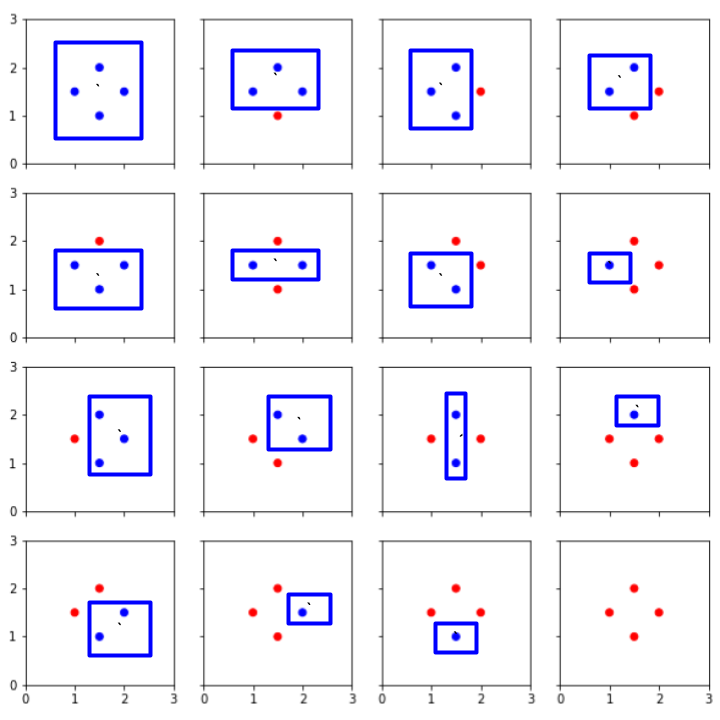
\includegraphics[scale=0.5]{./img/part3_2a1.png}
  	
  	\item ~Proof by contradiction for $VC(H^2_{rec}) < 5$:
  	For $VC(H^2_{rec}) >= 5$, there must exist at least one subset of size 5 that is shattered by $H^2_{rec}$. Let there be a set of four points $p_1, p_2, p_3, p_4,$ and $p_5$. Now consider two cases, case 1 where four points are enclosed and case 2 where only three points are within the rectangle.
  	\begin{enumerate}
  		\item[1.]{\textbf{Case 1:}} ~Let's assume that an axis-aligned rectangle correctly classifies $p_1, p_2, p_3$ and $p_4$ as positive and leaves $p_5$ outside the rectangle (labeled as negative). However, we can relabel the points such that 
  		$p_5$ is inside the rectangle, while the other four points are outside. This contradicts the assumption that the rectangle correctly classifies the points.
  		
  		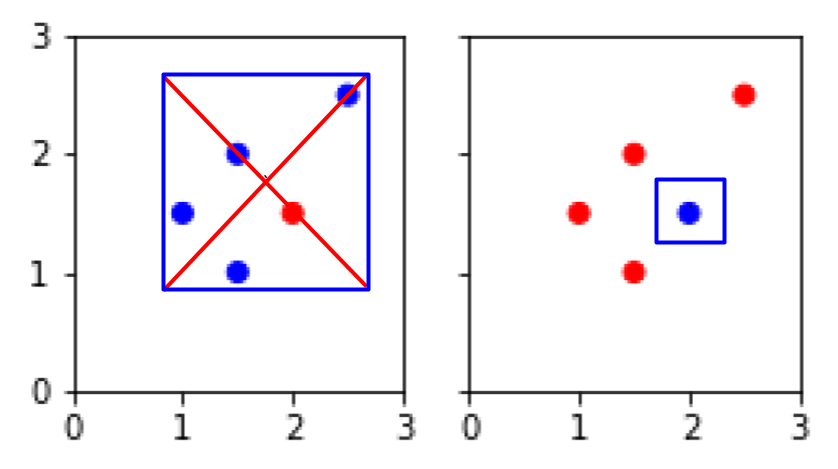
\includegraphics[scale=0.4]{./img/part3_2a2.png}
  		
  		\item[2.]{\textbf{Case 2:}} ~If an axis-aligned rectangle correctly classifies three points ($p_1, p_3,$ and $p_5$) as positive and two points as negative (remaining points), we can rearrange the points such that $p_2$ and $p_4$ are inside the rectangle while the rest are outside. Again, this contradicts the assumption.
  		
  		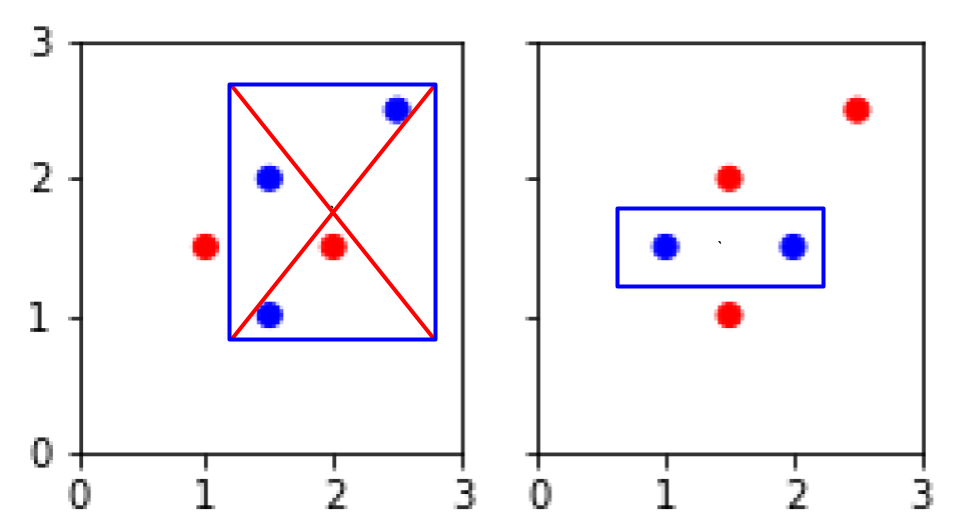
\includegraphics[scale=0.35]{./img/part3_2a3.png}
  	\end{enumerate}
  	Since no single rectangle can correctly classify all possible labelings of these five points, it's impossible to shatter a set of five points in $\mathbb{R}^2$.
  \end{enumerate}
  
  \item ~[10 points] Generalize your argument from the previous proof
    to show that for $d$ dimensions, the VC dimension of $H^d_{rec}$
    is $2d$.
    
	\textbf{Response:} To generalize on d-dimensions $H^d_{rec}$ must shatter at least one subset of size $2d$ (ie, $VC(H^d_{rec}) \geq 2d$) but there must not exist a single subset of size $2d+1$ that $VC(H^d_{rec})$ can shatter so $VC(H^d_{rec}) < 2d+1$.
	\newline
	Consider a set of points, each characterized by $d$ attributes. Each attribute can be positively or negatively labeled for each point. When we examine any subset of these points, we can always identify a rectangle that exclusively encompasses those points and not others. This observation establishes that the VC-dimension is at least $2d$. Now, let’s establish that the VC-dimension is less than $2d+1$. Visualize another set of points, this time focusing on the smallest rectangle that encompasses all these points. Given that we have more than $2d$ points, at least one point must reside within this rectangle. If we designate this interior point as "negative," no rectangle can effectively isolate it from the other points outside the rectangle. Hence, this demonstrates that the VC-dimension is less than $2d+1$. Combining these insights, we conclude that the VC-dimension equals $2d$.
  \end{enumerate}
  
\item In the lectures, we considered the VC dimensions of infinite
  concept classes. However, the same argument can be applied to finite
  concept classes too. In this question, we will explore this setting.

  \begin{enumerate}
  \item ~[10 points] Show that for a finite hypothesis class
    $\mathcal{C}$, its VC dimension can be at most
    $\log_2\left(|\mathcal{C}|\right)$. (Hint: You can use
    contradiction for this proof. But not necessarily!)
    
    \textbf{Response:} Suppose the finite concept class $C$ has a VC-dimension $d$ larger than $lg(|C|)$, then $d > lg(|C|)$. However, $2^d > |C|$ implies that are more unique labelings than $C$ contains as a finite concept class. Therefore, the VC-dimensions of a finite hypothesis class can be at most $lg(|C|)$.  

  \item ~[5 points] Find an example of a class $\mathcal{C}$ of
    functions over the real interval $X = [0,1]$ such that
    $\mathcal{C}$ is an {\bf infinite} set, while its VC dimension is
    exactly one.
    
    \textbf{Response:} The concept class under consideration involves half intervals. As demonstrated in the lecture, the hypothesis class consists of intervals on the real axis: $[a, b]$ where $a$ and $b$ are real numbers and $b > a$. In this specific instance, $a = 0$ and $b = 1$. It has been established that while there exists a dataset of size 1 that can be shattered, no dataset of size 2 can be fully classified.

  \item ~[5 points] Give an example of a {\bf finite} class
    $\mathcal{C}$ of functions over the same domain $X = [0,1]$ whose
    VC dimension is exactly $\log_2(|\mathcal{C}|)$.
	
	\textbf{Response:} The collection of disjoint sub-intervals is a finite class within the interval [0, 1]. It partitions the interval into discrete, equal segments, rendering it finite. By assigning a value of +1 to points residing within the intervals of this partition and -1 to those outside of it, complete classification can be achieved.
	
	It can be readily proven that the VC dimension is $lg(|C|)$. This is because we can easily shatter two points if they fall within one of these intervals. Moreover, all possible labelings can be attained by executing the various combinations of $|C|$ labelings.
  \end{enumerate}
  
\end{enumerate}
